%% This is the main content about this article. I should list them in an order
%% How to balance the existing model, positive and negative instance together, I shall use the dfg-method to create a dfg-matrix to incorporate the impact.
%% how to introduce them into adding long-term dependency feature. After mining the model by Inductive Miner, we have a model without long-term dependency, but we need to change the model and give the right examples.. 
%% If we change the data set, then we need to change the model into another parts, but the current methods can not solve it..
%% Should we also separate them into different sections?? Yes, we need it
%% Also, to delete the silent transition, as one option feature in our methods, we only delete it, in this situation, which will not affect the model behavoirs.

%% Or we could organize the content in this way:
%%  -- put the whole structure ahead and put all that we want to talk
%%  -- list the steps 
%%    ++ dfg-method to balance the directly-follows relation and create the corresponding directly-follows graph
%%    ++ add long-term dependency on the model
%%    ++ delete the silent transitions on the model as a post model

%% Put some words here
This chapter begins with a general framework to repair a reference model by incorporating the negative instances. In subsequent sections, we propose a concrete solution to implement the modules in the framework. 
%our repair algorithm to incorporate the negative instances on process enhancement. In the beginning, the architecture of this algorithm is provided to give an overview. Details of main steps are represented in the following order. Firstly, the impact of the existing model, positive and negative instances are balanced in the media of the directly-follow relations. Inductive Miner is then applied to mine process models from those directly-follows relations. Next, we detect and add long-term dependency on the generated process models. Furthermore, the model in Petri net with long-term dependency is  post-processed for the sake of simplicity. 
\section{General Framework}
%% Describe the 
Figure \ref{fig:framework} shows our proposed framework to repair a process model with negative information. The inputs are a reference process model and an labeled event log. The reference process model can be in multiple types, like Petri net, process tree. Traces in the labeled event log are classified as positive or negative in respect to some KPIs of business processes. The output is a repaired process model with the same type as the reference model.

The basic idea behind the framework is to unify the impact from the reference model $M$, positive sublog $L^+$ and negative sublog $L^-$ into data models. Those data models are of the same type and denoted as $D^M$, $D^+$ and $D^-$ respectively. Then we consider all impact from models and generate a new data model $D^n$. $D^n$ is later transformed into a process model $M^r$ as the output. Several post-processes are optional to improve the repaired model $M^r$.

After defining a data model to unify the impact and implementing the process modules in the general framework, a solution to repair model which also considers the negative information is able to find. 
\begin{figure}
	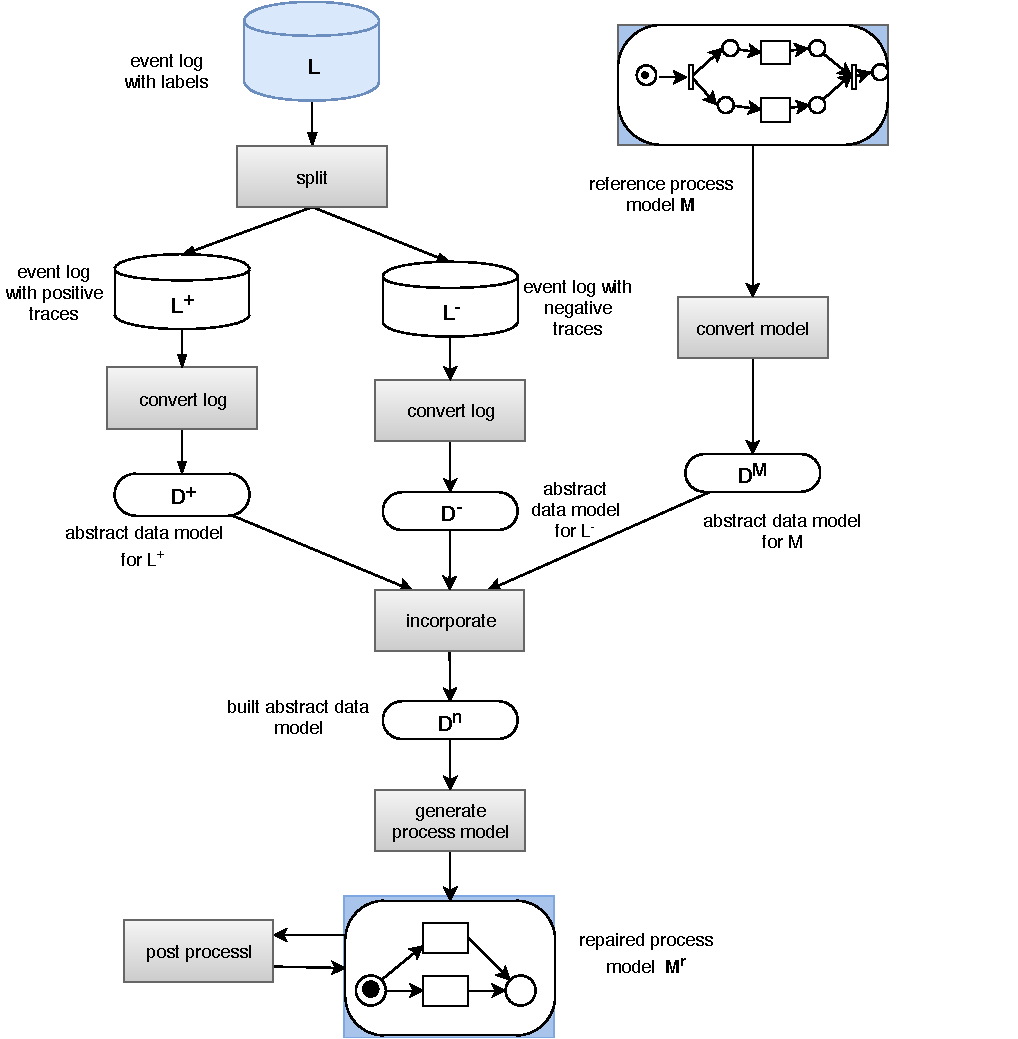
\includegraphics{figures/algorithm/FD_framework.pdf}
	\caption[Model Repair Architecture]{Model Repair Architecture -- \small Rectangles represents processes and data models in eclipse shape. Input event log and the reference model are in blue. Output in blue is a repaired model with the same type as the reference model.}
	\label{fig:framework}
\end{figure} 
\section{Algorithm}
Given the inputs as shown in the problem scope Figure \ref{fig:scope}, an event log and a Petri net as the reference process model M, we repair the Petri net with actual data in the event log and output the repaired Petri net. 

Based on those input and the condition with output, we give our algorithm to implement the modules to repair the reference Petri net. First of all, we define a proper data model to represent the impact from Petri net M, and the event log L. Then, we list all the modules  and describe our basic ideas to implement them. 
% here to point out our input and output
\subsection{Unified Data Model}
We choose directly-follows graph as the basis of our unified data model to represent the impact from the reference model and the event log. The reasons are, (1) directly-follows relation for building a directly-follows graph can be obtained from an event log and a reference model;(2) the cardinality of directly-follows graphs can be used to express the impact strength; (3) there exist transformation algorithms to extract a directly-follows graph from an event log and to convert directly-follows graph into process tree or Petri net, which saves our effort.

Although we can derive three directly-follows graphs from the reference model, the positive and negative event logs respectively, their cardinalities are in different level and disable to incorporate with each other. So we introduce a concept called unified cardinality to bring all the impact into the same level, which is the percentage to the sum of total cardinalities with a range [0-1].
% here we already changed the definitions for the unifications..now it became as the percentage of the cardinality to its whole cardinality. No matter negative or positive ones...we can do it, right? 
\begin{definition}[Unified cardinality] 
	\label{def:car-unification}
	Given a directly-follows graphs $G(L)  = (A, F , A_{start}, A_{end})$ for a model, the unification for this graph is a function  $u:F\rightarrow N $ that has the following definition: \\
	for each directly-follows relation $(a,b) \in F$,
	\[ u(a,b) = \frac{c(a,b)}{\sum_{(a^\prime,b^\prime) \in F} c(a^\prime,b^\prime)}\]
	for start activities $a \in A_{start}$, 
	\[ u(a) = \frac{c(a)}{\sum_{a^\prime \in A_{start}} c(a^\prime)} \]
	Similarly for end activities $a \in A_{end}$,
	\[ u(a) = \frac{c(a)}{\sum_{a^\prime \in A_{end}} c(a^\prime)} \]
\end{definition}
A directly-follows graph with unified cardinality is denoted as a unified directly-follow graph $D(L)=(A, F , A_{start}, A_{end}, u)$. After analyzing the positive , negative instances from event logs and the reference process model, $D(L_{pos})$, $D(L_{neg})$ and $D(L_{ext})$ are generated as the directly-follows graphs with unified cardinalities.
\subsection{Modules List}
After fixing the unified data models, in order to repair the reference model, the following list of modules are necessary. 
% should we add some steps here to say from which model to which model??
\begin{itemize}
	\item \emph{Split event log into positive and negative sublogs } \quad
	The event log $L$ is split into an event log $L^+$ with only positive traces and an event log $L^-$with negative traces.
	\item \emph{Convert event logs into unified directly-follows graphs, $D^+, D^-$}\quad 
	Two unified directly-follows graphs are generated respectively for the positive instance and negative instances from the event log.
	\item \emph{Convert process model into unified directly-follows graph $D^M$}\quad 
	\item \emph{Incorporate unified directly-follows graphs} \quad
	Three unified directly-follows  graphs $D^M, D^+, D^-$ are combined into one single directly-follows graph $D^n$ after balancing their impact.
	\item \emph{Generate process models from $D^n$} \quad
	Process models are mined from the repaired data model $D^n$.
	\item \emph{Post process the process model} \quad
	Several post-processes on the generated process model are optional to conduct, in order to improve the process model quality according to certain criteria.
	%Long-term dependency is detected on the intermediate models and finally added on the Petri net. To simplify the model, the reduction of silent transitions can be applied at the end.
\end{itemize}
In those modules, due to the simplicity, we skip the detail for the module \emph{Split event log into positive and negative sublogs}. The details of the concrete algorithms to implement other modules are provided in the subsequent sections.
\subsection{Convert event logs into unified directly-follows graphs, $D^+, D^-$}
Given an event log, to retrieve its unified directly-follows graph, we need to obtain its directly-follows graph at first. There is an existing procedure \emph{IMLog2Dfg} from \cite{leemans2013discovering}. \emph{IMLog2Dfg} traverses traces in the event log, extracts directly-follows relations of activities, and generates a directly-follows graph based on those relations. 

By applying \emph{IMLog2Dfg} separately on the event logs $L^+$ and $L^-$, we generate two directly-follows graphs $G(L_{pos})$ and $G(L_{neg})$.  In the next step, the cardinalities from those graphs are unified according to Definition \ref{def:car-unification} and become a part of unified data model $D(L_{pos})$ and $D(L_{neg})$

\subsection{Convert process model into unified directly-follows graph $D^M$}
The basic idea behind this convert is to transform a reference process model into a directly-follows graph and then unify this directly-follows graph into $D^M$.


To generate a directly-follows graph from a Petri net, we gather the model behaviors which are expressed in a transition system. By checking the transition system, directly-follows relations between activities are extracted and used later to a directly-follows graph for the reference model.

From the positive and negative event logs, we can get the cardinality for corresponding directly-follows graph to represent the strength of this directly-follows relation. However, when the existing model is transformed into  directly-follows graph $G(L_{ext})$, there is no point to assign cardinality on each edge. So we just set cardinality with 1 for each arc. Based on this cardinality assignment, we attain the unified data model $D^M$ for the reference Petri net.

\subsection{Incorporate unified directly-follows graphs}
After the unification, impact from existing model, positive and negative instances is in the same level and separately represented in $D^M$,$D^+$, and $D^-$. 
% explaination why we do Dm + D+ - D-, no need to have this, we can put the filtering step here, I will say..
To repair a reference model w.r.t. an actual event log with labels based on directly-follows relation, the strategy is that we add directly-follow relations into the repaired data model $D^n$ if the total support from $D^M$ and $D^+$ exceeds the rejection force from $D^-$; else, we reject directly-follows relations into the repaired model $D^n$. In other words, we balance all impact by subtracting the unified cardinality of $D^-$ from the sum of unified cardinality in $D^M$ and$D^+$.
\begin{definition}[Incorporating method] For any directly-follows relation from $D^M$,$D^+$, and $D^-$, we balance all forces on it in the following way. 
	\begin{itemize}
		\item For one directly-follows relation, \[ u^{n}(a,b) =  u^{M}(a,b)+ u^{+}(a,b)  - u^{-}(a,b) \] 
		\item For a start activity $a \in A^{M}_{start} \cup A^{+}_{start} \cup A^{-}_{start}$,
		\[ u^{n}(a) =  u^{M}(a)+ u^{+}(a)  - u^{-}(a)\]
		\item For an end activity $a \in A^{M}_{end} \cup A^{+}_{end} \cup A^{-}_{end}$
		\[ u^{n}(a) =  u^{M}(a)+ u^{+}(a)  - u^{-}(a)  \]
	\end{itemize}	
%if $u^{n}(a,b) > 1 , u^{n}(a,b) =1$, if $u^{n}(a,b) < 0 , u^{n}(a,b) =0$; 
% $ u^{n}(a) > 1 \Rightarrow  u^{n}(a) =1 ; u^{n}(a) < 0 \Rightarrow  u^{n}(a) =0$;
\end{definition}
% here is only the incorporation method
%% Here we add the control weight on it
In the real life, there exists various needs to address the impact either from the existing model, the positive instances or the negative instances. To meet this requirement, three control parameters $w^{M}$,$w^{+}$, and $w^{-} \in [0,1]$ are assigned respectively to each unified cardinality from the existing model, and positive and negative instances. The weighted unification is modified in the way bellow. 
\begin{definition}[Weighted incorporating method]
Given the control weight $w^{M}$,$w^{+}$, and $w^{-} \in [0,1]$, the weighted incorporating method to balance forces from $D^M$,$D^+$, and $D^-$ for $D_{n}$ is defined below.
\begin{itemize}
	\item For one directly-follows relation, \[ u^{n}_{w}(a,b) =  w^{M} * u^{M}(a,b)+ w^{+} * u^{+}(a,b)  - w^{-} * u^{-}(a,b) \] 
	\item For a start activity $a \in A^{M}_{start} \cup A^{+}_{start} \cup A^{-}_{start}$,
	\[ u^{n}(a) =  w^{M} * u^{M}(a)+ w^{+} * u^{+}(a)  - w^{-} * u^{-}(a)\]
	\item For an end activity $a \in A^{M}_{end} \cup A^{+}_{end} \cup A^{-}_{end}$
	\[ u^{n}(a) =  w^{M} * u^{M}(a)+ w^{+} * u^{+}(a)  - w^{-} * u^{-}(a)  \]
\end{itemize}	
\end{definition}
By adjusting the weight of $w^{M}$,$w^{+}$, and $w^{-}$, different focus can be reflected by the model. For example, by setting $w^{M}=0, w^{+}=1,w^{-}=1$, the existing model is ignored in the repair, while  the original model is kept in situation $w^{M}=1, w^{+}=0,w^{-}=0$.

Next, we filter the directly-follows relation according to its weighted cardinality. If the cardinality over one certain threshold, it indicates a significant support to add this relation into the repaired data model $D^n$. By adding those directly-follows relation, we build a unified directly-follow graph $D^n$ over this threshold t. The algorithm is listed in Algorithm ??. 
\begin{algorithm}[H]
	\SetAlgoLined
	\KwResult{The repaired data model $D^n$}
	$D^n=(A=\emptyset, F=\emptyset , A_{start}=\emptyset, A_{end}=\emptyset,u=\emptyset)$\;
	Given a threshold $t \in [0,1]$, 
	the weighted unified cardinality set from $D^M$,$D^+$, and $D^-$, \quad 
	$U^{n}:F^{M} \cup F^{+} \cup F^{-} \rightarrow \mathbb{R}$\;
	\For{Each weighted unified cardinality $u^n(a,b)$}{
		\If{$u^n(a,b)$ > t}{
			\If{$u^n$ > 1.0}{
				$u^n$ = 1.0
		    }
	    	$A=A\cup \{a\} \cup\{b\}$ \;
			$F=F\cup \{(a,b)\}$ \;
			$u=u\cup \{(a,b) \rightarrow u^{n}\}$;
		}
	}
	\For{Each weighted unified cardinality for the start activity $u^n(a)$}{
		\If{$u^n(a)$ > t}{
			\If{$u^n$ > 1.0}{
				$u^n$ = 1.0
			}
		    $A = A\cup\{a\}$\;
			$A_{start}=A_{start}\cup \{a\} $ \;
			$u=u\cup \{(a) \rightarrow u^{n}\}$\;
		}
	}
	\For{Each weighted unified cardinality for the end activity $u^n(a)$}{
		\If{$u^n(a)$ > t}{
			\If{$u^n$ > 1.0}{
				$u^n$ = 1.0
			}
			$A = A\cup\{a\}$\;
			$A_{end}=A_{end}\cup \{a\} $ \;
			$u=u\cup \{(a) \rightarrow u^{n}\}$\;
		}
	}
	\caption{Build data model $D^n$ after incorporating $D^M$,$D^+$, and $D^-$ }
\end{algorithm}
% here to explain the building method for the new data model and the way from it?? But should we do it here, or later?? 
%After getting the weighted unification, we can assign cardinality for the directly-follows graph $G_{new}$ by multiplying weighted unification with the total number of cardinalities of $G(L_{pos})$, $G(L_{neg})$ and $G(L_{ext})$. 
\subsection{Generate process models from $D^n$}
% generate dfg from unified one
% derive models from dfg
The result from the last step above is a unified directly-follows graph $D^n$ with weighted cardinality. To generate a process model from it, we convert $D^n$ firstly into a general directly-follows graph $G^n$. Analyzing the weighted cardinality, we know all of them are in range [0,1]. We transform the weighted cardinality by multiplying the sum of cardinalities of $G(L^{+})$, $G(L^-)$ and $G(L^{M})$.  


Later, based on $G^n$, an existing procedure called \emph{Dfg2ProcessTree} is applied to mine process models like process tree and Petri net.  This procedure was introduced with Inductive Miner\cite{leemans2013discovering}. It finds the most prominent split from the set of exclusive choice, sequence, parallelism, and loop splits on  a directly-follows graph.  Afterward, the corresponding operator to the split is used to build a block-structured process model called a process tree. Iteratively, the split sub graphs are passed as inputs for the same procedure until one single activity is reached and no split is available. A process tree is output as the mined process model and can be converted into another process model called Petri net.
%% To write the procedure for it 

\subsection{Post process on the process model}
Due to the intrinsic characters of Inductive Miner, the dependency from activities which are not directly-followed can't be discovered. To make the generated model preciser, as one post process, we detect the long-term dependency and add it on the process model.  What's more, to simplify the model, we can delete redundant silent transitions and places as another post process.  
\subsubsection{Add long-term dependency}
Obviously, long-term dependency relates the structure of choices in process model, such as exclusive choice, loop and or structure. Due to the complexity of or and loop structure, we only deal with the long-term dependency in the exclusive choice structure. 

To analyze the exclusive choice structure, we use process tree as an intermediate process model due to several reasons: (1) easy to extract the exclusive choice structure from process tree, since process tree is block-structured. (2) easy to transform a process tree to a Petri net. 
%% Here we need to add the relation of process to the long-term dependency

An exclusive choice structure be represented as \textbf{\emph{xor block}} in a process tree. For the sake for convenience, we name a subtree of an xor block as one \textbf{\emph{xor branch}}, and denote the set of xor blocks B(Q) as and the set of xor branches as BB(Q) for a tree Q.
For two arbitrary xor branches with long-term dependency, they have to satisfy the conditions: (1) they have a sequential order;(2) they have significant correlation.
The order of xor branch follows the same rule of node in process tree which is explained in the following.
\begin{definition}[Order of nodes in process tree]
	Node $X$ is before node $Y$, written in $X \prec Y$, if $X$ is always executed before $Y$.  In the aspect of process tree structure, $X \prec Y$, if the least common ancestor of $X$ and $Y$ is a sequential node, and $X$ positions before $Y$.
\end{definition} 

The correlation of xor branches is significant if they always happen together. To define it, several concepts listed below are necessary. 
\begin{definition}[Xor branch frequency]
	The frequency for an xor branch $X$ in event log L is the count of traces, $f: X \rightarrow N$.   
	\[f_{L}(X) = \sum_{\sigma \in L} |\{\sigma \vert \sigma \models X\} |\]
	For multiple xor branches, the frequency of their coexistence in event log L is defined as the count of traces with all the occurrence of xor branches ${Xi}$ , \[f_{L}(X_1, X_2,...,X_n)= \sum_{\sigma \in L} |\{\sigma \vert \forall X_i, \sigma \models X_i\} | \]
\end{definition}
The frequency of the coexistence of multiple xor branches in positive and negative event logs reflects the correlation of those xor branches. The long-term dependency in the existing model also affects the long-term dependency in the repaired model. However, since the repaired model possibly differs from the existing model, the impact of long-term dependency from the existing model becomes difficult to detect. With limits of time, we only consider the impact from positive and negative instances on the long-term dependency.
%In one way, it has explicit long-term dependencies that should be kept. In another way, the existence of xor branches implies a full-connected long-term dependency. To incorporate the influence from the existing model, we give the definition for xor branch correlation.
% but to detect the explict long-term dependency, we need one pre-process?? But how ?? Also, how to combine the effect into the model then??
%% To detect it:: <1> xor blocks in the Petri net,  1.0 is assigned to the existing model but, but !!! we can not decide it!! Because the xor block the generated model differs from the existing models!! So our whole methods can have such wrong parts!! If the wrong part from them, we need to make sure the xor branches also exist in the repaired model. Then we need to check the long-term depedency. We must see the positive and negative ones..
% so we can also have the positive and negative instances for long-term dependency.
%% combine the existing model factor together. How about we record the long-term dependency from the existing model?? How to extract the long-term dependency from the model?? No method currently
\begin{definition}[Correlation of xor branch] The correlation to express dependency of two branches $X,Y \in BB(Q)$ is expressed into
	\[d(X,Y)=  d^{+}(X, Y) -d^{-}(X, Y)\], where 
	\[d^{+}(X, Y)= \frac{f_{L^+}(X, Y)}{\sum_{Y^\prime BB(Q), Y^\prime \neq X} f_{L^+}(X, Y^\prime)}, \quad d^{-}(X, Y)= \frac{f_{L^-}(X, Y)}{\sum_{Y^\prime BB(Q), Y^\prime \neq X} f_{L^-}(X, Y^\prime)}\]	
\end{definition}
$f_{L^+}(X, *) $ and $f_{L^-}(X, Y)$ are the frequency of the coexistence of $X$ and $Y$, respectively in positive and negative event logs.
% here we need to define the long-term dependency
%Based on the concepts above, we give a formal definition for long-term dependency in this thesis. 
%\begin{definition}[Long-term dependency for xor blocks] We call two xor blocks $S=\{X_1,X2,...X_m\}$ and $T=\{Y_1,Y_2,...Yn\}$ with long-term dependency, if 
%	 \[ S \prec T, d  \]
%\end{definition}
\subsubsection{Cases Analysis}
% Here we need to check the combination for all xor branches, but with one example.
There are various sorts of long-term dependencies that are able to happen for two xor blocks. To explain those situations better, we define concepts called sources and targets of long-term dependency and then give an example of one Petri net with long-term dependency.
\begin{definition}[Source and target set of Long-term Dependency]
	The source set of the long-term dependency in two xor blocks is the set of all  xor branches, $LT_S:= \{X \vert \exists Y, X\rightsquigarrow Y  \in LT \} $, and target set is $LT_T:= \{Y \vert \exists X, X\rightsquigarrow Y \in LT \} $. \\
	For one xor branch $X \in S$, the target xor branch set relative to it with long-term dependency is defined as:
	$ LT_T(X)= \{Y \vert  X\rightsquigarrow Y \in LT \}$
	Respectively, the source xor branch relative to one xor branch in target is
	$ LT_S(Y)= \{X \vert  X\rightsquigarrow Y \in LT \}$
\end{definition}
At the same time, we use $S $ and $T$ to represent the set of xor branches for source and target xor block with long-term dependency.
Given an Petri net in Figure \ref{fig:seq-2-original}, two xor blocks are contained in the model which allows the following long-term situations.
\begin{figure}
	\centering
	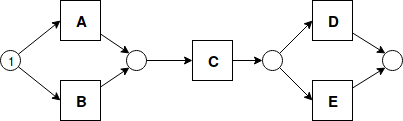
\includegraphics[width=\linewidth]{figures/algorithm/LT_Seq_01_Original.png}
	\label{fig:seq-2-original}
	\caption{One Petri net with two two xor blocks}
\end{figure}
\begin{enumerate}
	\item $LT=\{ A\rightsquigarrow D, A\rightsquigarrow E, B\rightsquigarrow D, B\rightsquigarrow D\}$. \\
	$LT_S = \{A,B\}, LT_T=\{D,E\}, \vert LT \vert = \vert S \vert * \vert T \vert  $, which means long-term dependency has all combinations of source and target xor branches. 
	\item $LT=\{ A\rightsquigarrow D, A\rightsquigarrow E, B\rightsquigarrow E\}. $\\
	$LT_S = \{A,B\}, LT_T=\{D,E\}$
	$LT_S = S $ and $LT_T = T, \vert LT \vert < \vert S \vert * \vert T \vert $. it doesn't cover all combinations. But for one xor branch $X \in S, LT_T(X)= T$, it has all the full long-term dependency with $T$. 
	\item $LT=\{ A\rightsquigarrow D, B\rightsquigarrow E\}. $\\
	$LT_S = \{A,B\}, LT_T=\{D,E\}$
	$LT_S = S $ and $LT_T = T, \vert LT \vert < \vert S \vert * \vert T \vert $. For all xor branch $X \in S, LT_T(X) \subsetneq T$, none of xor branch X has long-term dependency with $T$.
	\item $LT=\{ A\rightsquigarrow D, B\rightsquigarrow D\}.$ \\
	$LT_S = S ,  LT_T \subsetneq T$. There exists at least one xor branch $Y \in T$ which has no long-term dependency on it.
	\item $LT=\{ A\rightsquigarrow D, A\rightsquigarrow E\}.$ \\
	$LT_S \subsetneq S ,  LT_T = T$.
	There exists at least one xor branch in source $X \in S$ which has no long-term dependency on it.
	\item $LT=\{ A\rightsquigarrow E\}. $\\
	$LT_S \subsetneq S ,  LT_T \subsetneq T$.
	There exists at least one xor branch in source $X \in S$  and one xor target xor branch which has no long-term dependency on it.
	\item $ \emptyset$ . There is no long-term dependency on this set. 
\end{enumerate}
In the following, we propose a method to express long-term dependency on Petri net. 
%% should we write down here to prove the correctness of available situations, or we need to wait??
\subsubsection{Way to express long-term dependency}
Adding places to Petri net can limit the behavior\cite{bergenthum2007process}, since its output transitions demand a token from it to fire themselves. When there is no token at this place, the transitions are enabled. By injecting extra places on Petri net, it can block negative behaviors which are not expected in the aspect of business performance. 

Long-term dependency limits the available choices to fire transitions after the previous xor branch executes. So to express long-term dependency, our basic idea is to add places to the Petri net model. What's more, because one xor branch can be as a source to multiple long-term dependencies and one xor branch can be as a target to multiple long-term dependencies, silent transitions are also needed to address a long-term dependency explicitly. 


Given arbitrary two xor blocks, $S=\{X_1,X2,...X_m\}$ and $T=\{Y_1,Y_2,...Yn\}$ with long-term dependency $LT=\{X_i \rightsquigarrow Y_j \vert 1 \leq i \leq m, 1 \leq j \leq n \}$, we add places after the source xor branches,  $P_S=\{p_{X_i} \vert X_i \in LT_{S} \}$, and places before target xor branches,$P_T=\{p_{Y_j} \vert Y_i \in LT_{T} \}$. For each long-term dependency $X_{i} \rightsquigarrow Y_{j}$ in LT, there is silent transition t with $p_{X_i} \rightarrow t \rightarrow p_{Y_{j}}$. The steps to add silent transitions and places according to the long-term dependency are listed in algorithm \ref{alg: Adding method}.

% An algorithm is given to show how to add the long-term dependency
\begin{algorithm}[!ht]
	\SetAlgoLined
	$Y$ is dependent on $X$\;
	\If{$X$ is leaf node}{
		One place is added after this leaf node \;
	}
	\If{$X$ is Seq}{
		Add a place after  the end node of this branch\;
		The node points to the new place\;
	}
	\If{$X$ is And}{
		Create a place after the end node of every children branch in this And xor branch \; 
		Combine all the places by a silent transition after those places \;
		Create a new place directly after silent transition to represent the And xor branch \;
	}
	
	\If{$Y$ is leaf node}{
		One place is added before this leaf node \;
	}\If{$Y$ is Seq}{
		Add a place before  the end node of this branch\;
		The new place points to this end node\;
	}\If{$Y$ is And}{
		Create a place before the end node of every children branch in this And xor branch \; 
		Combine all the places by a silent transition before those places \;
		Create a new place directly before silent transition to represent the And xor branch \;
	}
	Connect the places which represent the $X$ and $Y$ by creating a silent transition.
	\caption{Add long-term dependency between pure xor branch}
	\label{alg: Adding method}
\end{algorithm}
\begin{figure}
	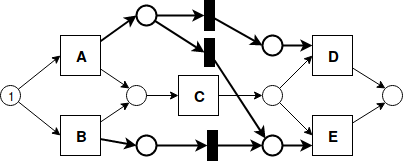
\includegraphics[width=\textwidth]{figures/algorithm/LT_Seq_01_Silent_01.png}
	\label{fig:add-algorithm-example}
	\caption{Model with long-term dependency $LT=\{ A\rightsquigarrow D, A\rightsquigarrow E, B\rightsquigarrow E\}. $ }
\end{figure}
One simple example is given in the Figure \ref{fig:add-algorithm-example} to explain this algorithm. Given the long-term dependencies $LT=\{ A\rightsquigarrow D, A\rightsquigarrow E, B\rightsquigarrow E\}$, two extra places are added respectively after A and B; Next, two places before D and E are created to express that the xor branches are involved with long-term dependency. At end, for each long-term dependency, a silent transition is generated to connect the extra places after the source xor branch to the place before target place. 

\subsubsection{Soundness Analysis}
% this section is used to select the sound situations. 
% next time I can go to library at Tuesday with the laptop and study there..
Following algorithm \ref{alg: Adding method} by adding silent transitions and places to express long-term dependency, the model soundness can be violated. In the following section, we discuss the soundness in different situations. 

Given a Petri net with long-term dependency $LT=\{X_i \rightsquigarrow Y_j \vert 1 \leq i \leq m, 1 \leq j \leq n \}$ on two xor blocks $S=\{X_1,X2,...X_m\}$ and $T=\{Y_1,Y_2,...Yn\}$, following the Algorithm \ref{alg: Adding method}, $P_S=\{p_{X_i} \vert X_i \in LT_{S} \}$ , $P_T=\{p_{Y_j} \vert Y_i \in LT_{T} \}$, and silent transitions $ E = \{\epsilon \vert p_{X_i} \rightarrow \epsilon
\rightarrow p_{Y_{j}} \}$ are added. 
 
The Petri net is sound if and only if (1)the soundness outside xor blocks with long-term dependency is not violated; and  (2) soundness between xor blocks is kept. In the following, we check the model soundness with long-term dependency after applying Algorithm \ref{alg: Adding method}. \\\\
\textbf{Soundness outside xor blocks.}\\
	\emph{Proof:} he added silent transitions and places do not violate the execution outside of the xor blocks, because the extra tokens that are generated due to long-term dependency are constrained in the xor blocks, and it doesn't affect the token flows outside. As we know, the original model is sound. So the soundness outside xor blocks is not violated.
%% begin to prove the soundness inside xor block
\\\\
\textbf{Soundness inside xor blocks.}\\
For all xor branches in S, only one branch can be fired. Without loss of generality, $X_i$ is assumed to be enabled. After firing $X_i$, the marking distribution on the extra places are  
\[ M(p_{X_i}) = 1; \quad 
\forall p_{X_i^\prime} \in P_S, i^\prime \neq i, M(p_{X_i^\prime})=0 \]
%% here we need to divide them into different situations...
If $ LT_S = S, LT_T=T$, adding the long-term dependency in this situation doesn't violate the model soundness, we prove it in the following part.
%the following conditions are checked. 
\begin{itemize}
	\item safeness. Places cannot hold multiple tokens at the same time.\\
	For all extra places $p_{X_i}$ and $p_{Y_j}$, 
	\[\forall p_{X_i} \in P_S, \sum M(p_{X_i})=1\]
	Because $ LT_S = S, X_i \in S$, so $X_i \in LT_S$, there exists one $Y_j$ with $X_i \rightarrow Y_j$ and one $\epsilon, p_{X_i} \rightarrow \epsilon
	\rightarrow p_{Y_{j}} $.  After firing $X_i$, the transition $\epsilon$ becomes enable. After executing $\epsilon$, the marking distribution turns to 
	\[ M(p_{Y_j}) = 1;\quad 
	\forall p_{Y_j^\prime} \in P_T, j^\prime \neq j,  M(p_{Y_i})=0 \]
	So whenever the marking distribution in the extra places are
	\[\sum M(p_{X_i}) \leq 1,  \sum M(p_{Y_j}) \leq 1 \] 
	\item proper completion. If the sink place is marked, all other places are empty. \\
	After firing $Y_j$, all the extra places hold no token. So it does not violate the proper completion.
	\item option to complete.  It is always possible to reach the final marking just for the sink place. \\
	There is always one $Y_j$ enabled after firing $X_i$ to continue the subsequent execution.
	\item no dead part. For any transition there is a path from source to sink place through it. \\
	Because all $Y_j \in T$ are also in $LT_T$, there exists at least one $X_i\in S$ with long-term dependency with $Y_j$. After $X_i$ is fired, one token is generated on the extra place $p_{X_i}$ and can be consumed by silent transition $\epsilon$ in  $p_{X_i} \rightarrow \epsilon \rightarrow p_{Y_{j}}$ to produce a token in $p_{Y_j}$, which enables xor branch $Y_j$ and leaves no dead part.
\end{itemize}
Else, in other situation, the model becomes unsound. \\
\indent If $LT_S \neq S,or\quad LT_T \neq \emptyset$, there exists one xor branch $X_i$ with $X_i \notin LT_S$. When $X_i$ is fired, it generates one token at place $p_{X_i}$, this token cannot be consumed by any $Y_j$. So it violates the proper completion. \\  
\indent If $LT_T \neq T$, there exists one $Y_j \notin LT_T, \nexists X_i, X_i \rightsquigarrow Y_j$, so with two input places but $Token(p_{Y_j})=0$,  $Y_j$ becomes the dead part, which violates the soundness again. \\

As a conclusion, to keep Petri net with long-term dependency sound, only situation $ LT_S = S, LT_T=T$ is considered. However, when the long-term dependency is full connected where each combination of xor branches from source and target xor block has long-term dependency, namely xor branches can be chosen freely, we don't add any places and silent transitions on the model. 
\subsection{Reduce Silent Transitions}
%% We reduce the silent transition when there is no 
Our method to represent long-term dependency can introduce redundant silent transitions and places, which complicates the model. So, we post process the Petri net with long-term dependency to delete redundant silent transitions and places.
% ; on the other hand, it causes the model unsound where the extra silent transitions suspend the execution and therefore violates the soundness condition of proper completion.
\begin{proposition}
	Given a silent transition $\epsilon$ in Petri net with one input place $P_{in}$ and one output place $P_{out}$, if $\vert Outedges({P_{in}) }\vert \geq 2 \quad and \quad \vert Inedges(P_{out}) \vert \geq 2 $, the silent transitions can not be deleted. Else, the silent transitions is able to delete, meanwhile the $P_{in}$ and $P_{out}$ can be merged into one place. This reduction does not violate the soundness and does not change the model behavior.
\end{proposition}
\begin{proof}[Soundness Proof]
	If a silent transition t is able to delete, then
	\[\vert Outedges({P_{in}) }\vert \leq 1	\quad (1) \quad or, \]
	\[\vert Inedges({P_{out}) }\vert \leq 1\quad (2).\]
	When in case (1), $P_{in}$ contains a token that is always passed to $P_{out}$ by silent transitions t. After deleting the silent transition, the token is generated directly on $P_{out}$. Since t is silent transition, it won't affect the model behavior. \\ 
	when in case (2), $P_{out}$ contains a token that is always passed from $P_{in}$ by silent transitions t. After deleting the silent transition, the token is remained on $P_{in}$, which enables the later execution after the original $P_{out}$. Since t is silent transition, it won't affect the model behavior. \\
	In other cases, $Outedges({P_{in}) }\vert \geq 2 \quad and \quad \vert Inedges(P_{out}) \vert \geq 2$, which means that the source xor branch with output place $P_{in}$ has at lest two long-term dependencies; the target xor branch with input place $P_{out}$ has at least two long-term dependencies. If we delete this silent transitions, the long-term dependencies are mixed together which allows more unexpected behaviors. Therefore, silent transition in this situation is necessary to hold long-term dependency.
\end{proof}
%% here we need to prove this proposition
One example is given in the following graph. $M_{lt}$ in Figure \ref{fig:with-lt} has long-term dependency expressed in the silent transitions and places. The silent transition for $S2 \rightsquigarrow B1 $ and silent transition for $B1 \rightsquigarrow T2$ belongs to the case (1). So they are kept in the model, while the other silent transitions are deleted. After reducing the redundant silent transitions, the model becomes $M_r$ shown in Figure \ref{fig:reduced-lt}. Those two models have the same behavior, yet the reduced model is simpler.
\begin{figure}[!h]
	\centering
	\begin{subfigure}[a]{\textwidth}
		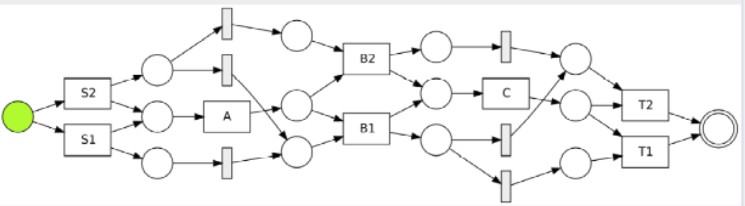
\includegraphics[width=\textwidth]{figures/algorithm/dfg-IM-pn-with-lt.png}
		\label{fig:with-lt}
		\caption{A Petri net $M_{lt}$ with redundant silent transitions}
	\end{subfigure}
	\hfill
	\begin{subfigure}[b]{\textwidth}
		\centering
		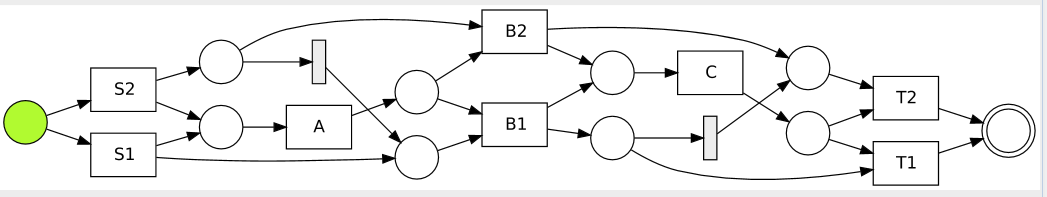
\includegraphics[width=\linewidth]{figures/algorithm/dfg-IM-pn-with-lt-reduced.png}
		\label{fig:reduced-lt}
		\caption{Petri net $M_r$ with reduced silent transitions}
	\end{subfigure}
\end{figure}
\subsection{Concrete Architecture}
At last, we assemble all the modules together and give an overview architecture of our repair techniques.  We reuse existing modules in gray rectangles in Figure \ref{fig:architecture}, e.g. IMLog2Dfg to convert an event log into directly-follow graph, Petrinet2TransitionSystem to transform a Petri net into a transition system. The other modules are programmed according to our specific needs and achieve the repair algorithm mentioned before. To achieve a preciser Petri net, the module to add long-term dependency becomes a necessary part. Yet, reduction on redundant places and silent transitions is optional. 
\begin{figure}
	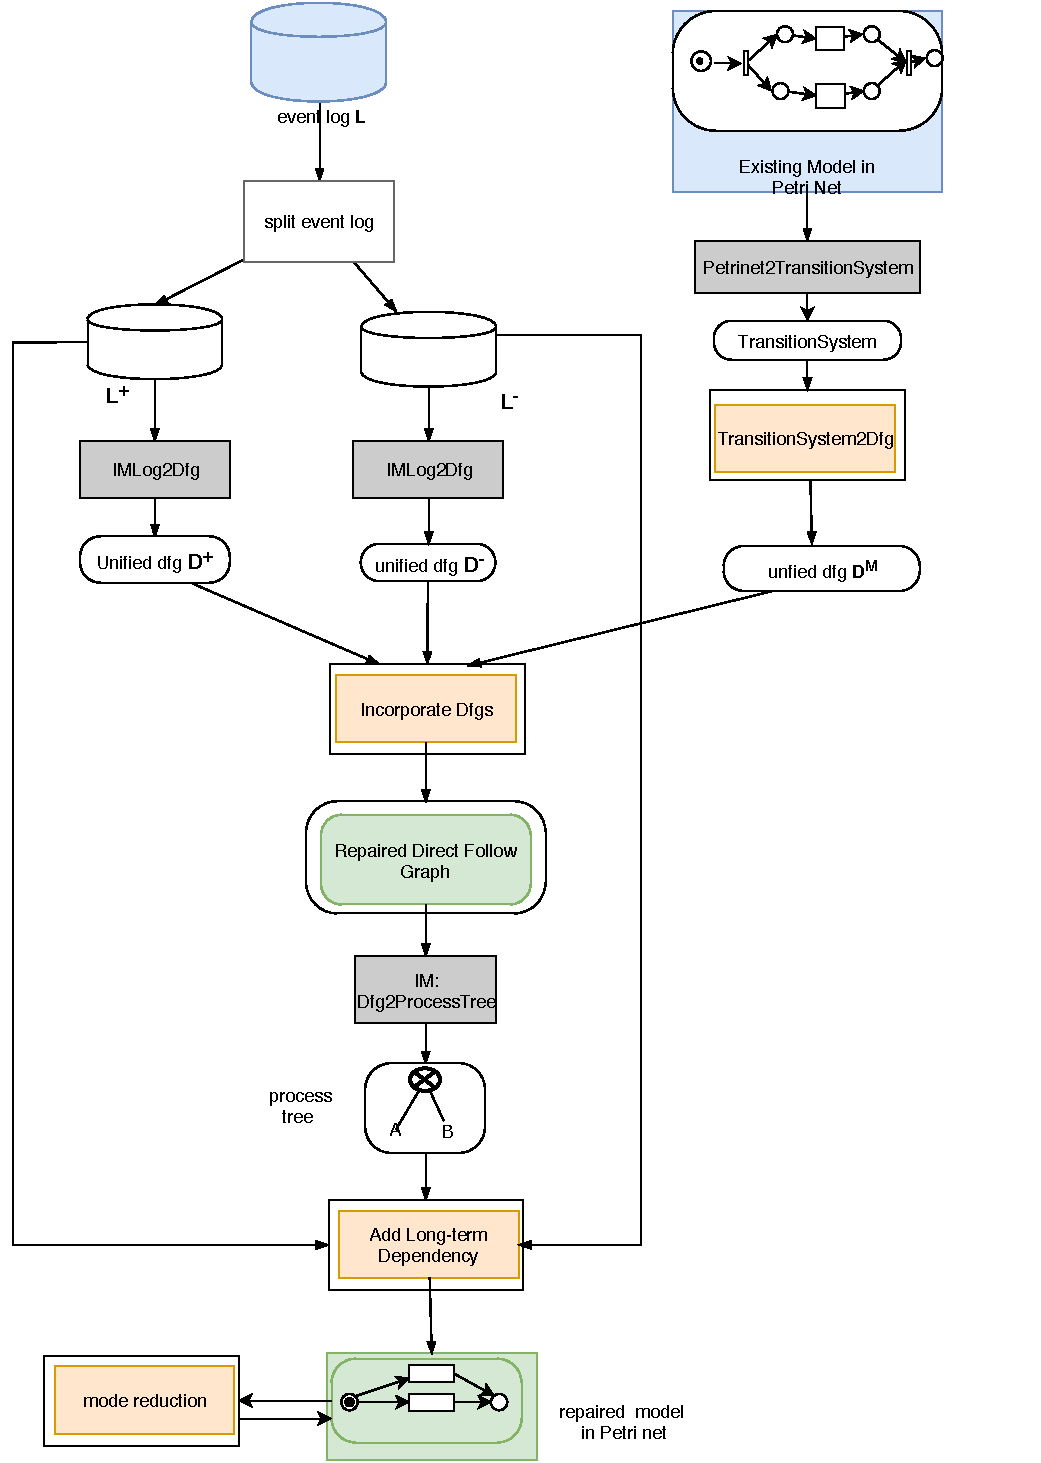
\includegraphics[height=0.9\textheight]{figures/algorithm/FD_architeccture_detail.pdf}
	\caption[Model Repair Architecture]{Model Repair Architecture -- \small Rectangles represents processes and output data in eclipse shape, especially customized processes and data are in doubled lattice shape. Input event log and existing model are in blue, KPIs are in cloud. The output is a petri net in purple.}
	\label{fig:architecture}
\end{figure} 
